% Preprocessing pipeline libraries - Library reference - Top level
% Written by Christopher Thomas.

\documentclass[letterpaper,11pt]{report}
\usepackage[letterpaper]{geometry}
\usepackage{graphicx}
\usepackage{verbatim}
\usepackage{placeins}
\usepackage{longtable}

\geometry{nohead,footskip=0.3in,margin=0.75in}

% Force my paragraph style, darnit.
\usepackage{indentfirst}
\setlength{\parskip}{\baselineskip}

% NOTE - "\thispagestyle" is used for part and chapter beginning pages, and
% overrides \pagestyle. Redefine it to be harmless.
% NOTE - The canonical solution ("\pagenumbering{gobble}") resets the page
% counter whenever it's used.
\renewcommand{\thispagestyle}[1]{}

% Custom macros.
\newcommand{\fixme}[1]{\textbf{FIXME: #1}}

\newcommand{\figdef}[3]
{\begin{figure}[htb]
\begin{center}#1\end{center}
\caption{#2}\label{#3}\end{figure}}

\newcommand{\tabdef}[3]
{\begin{table}[hb]
\begin{center}#1\end{center}
\caption{#2}\label{#3}\end{table}}

% Document body.
\begin{document}
%
% Title page.
%
\pagestyle{empty}

\begin{center}
%
\vspace*{1in}
{\LARGE Preprocessing Pipeline Libraries -- Function Reference} \\
{\footnotesize Written by Christopher Thomas -- \today.}
%
\vspace*{1in}\\
\begin{tabular}{cc}
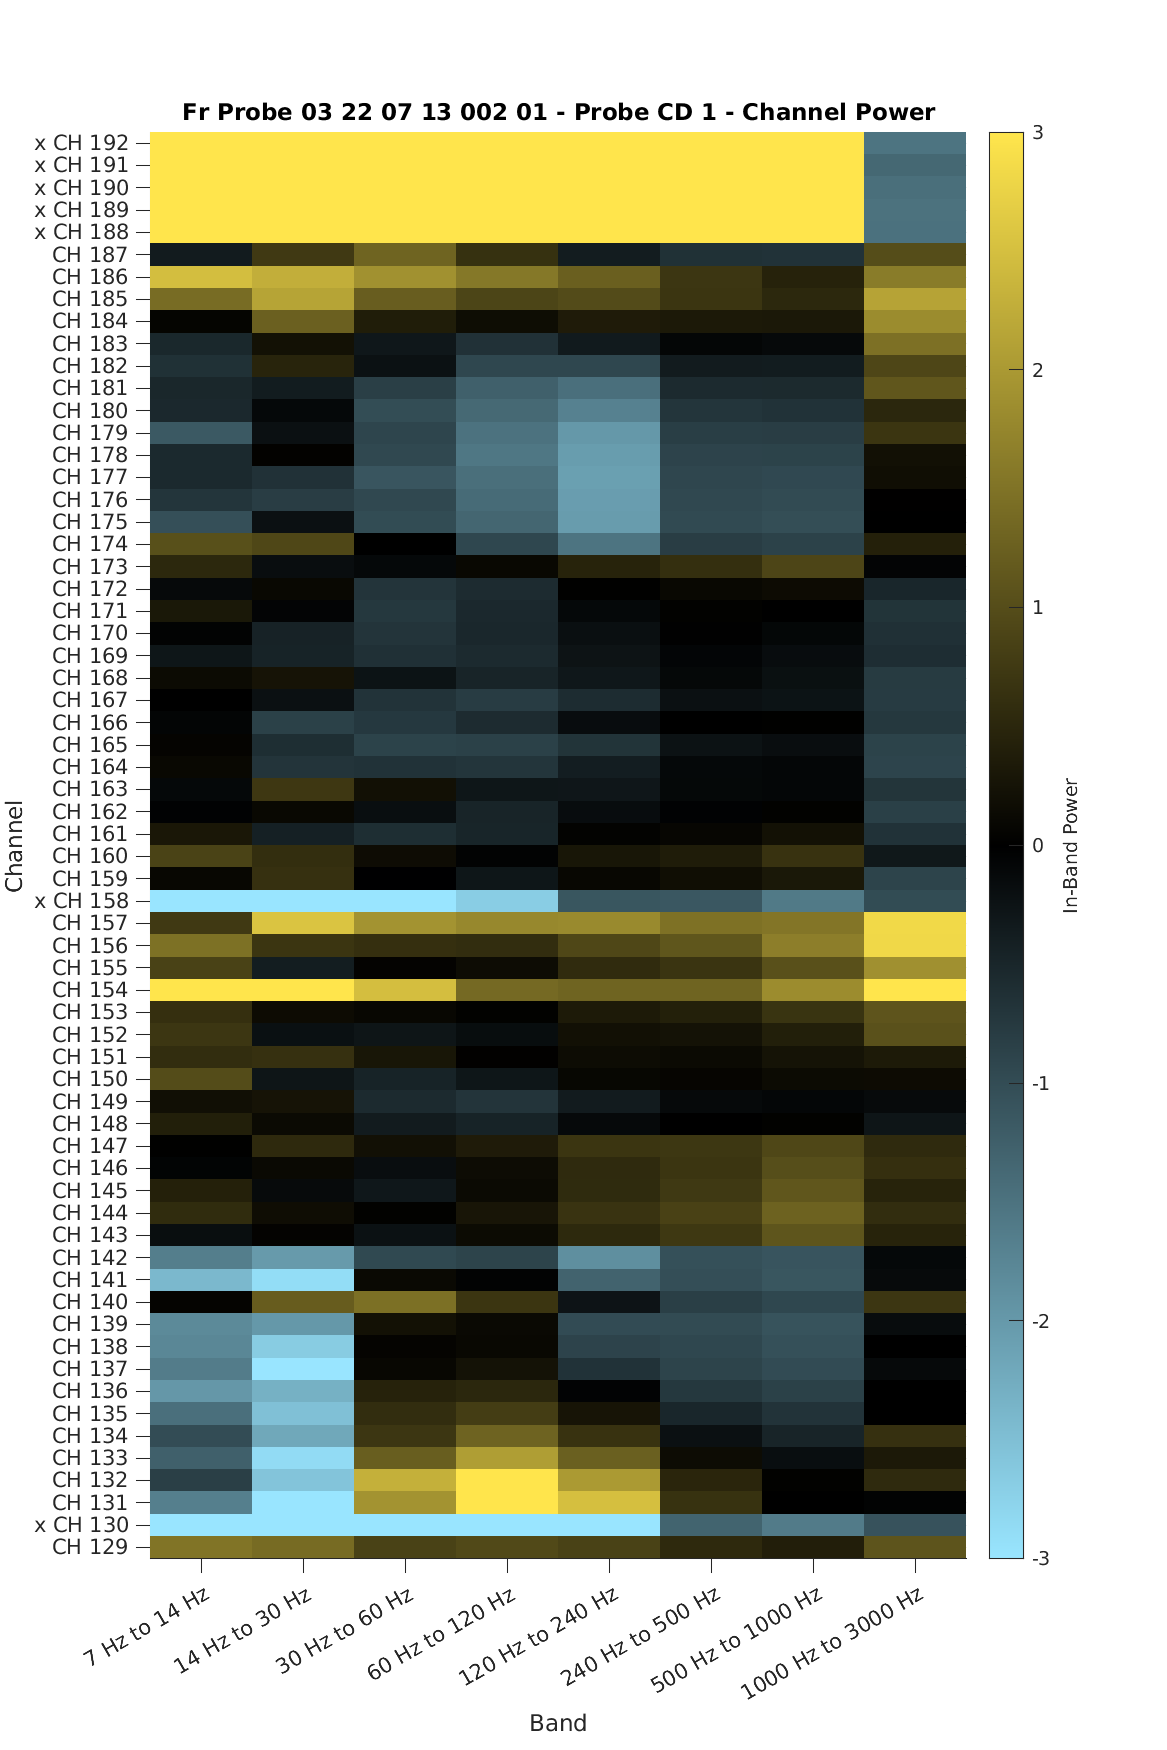
\includegraphics[width=3in]{plots/0713-prCD1-inband-normchan} &
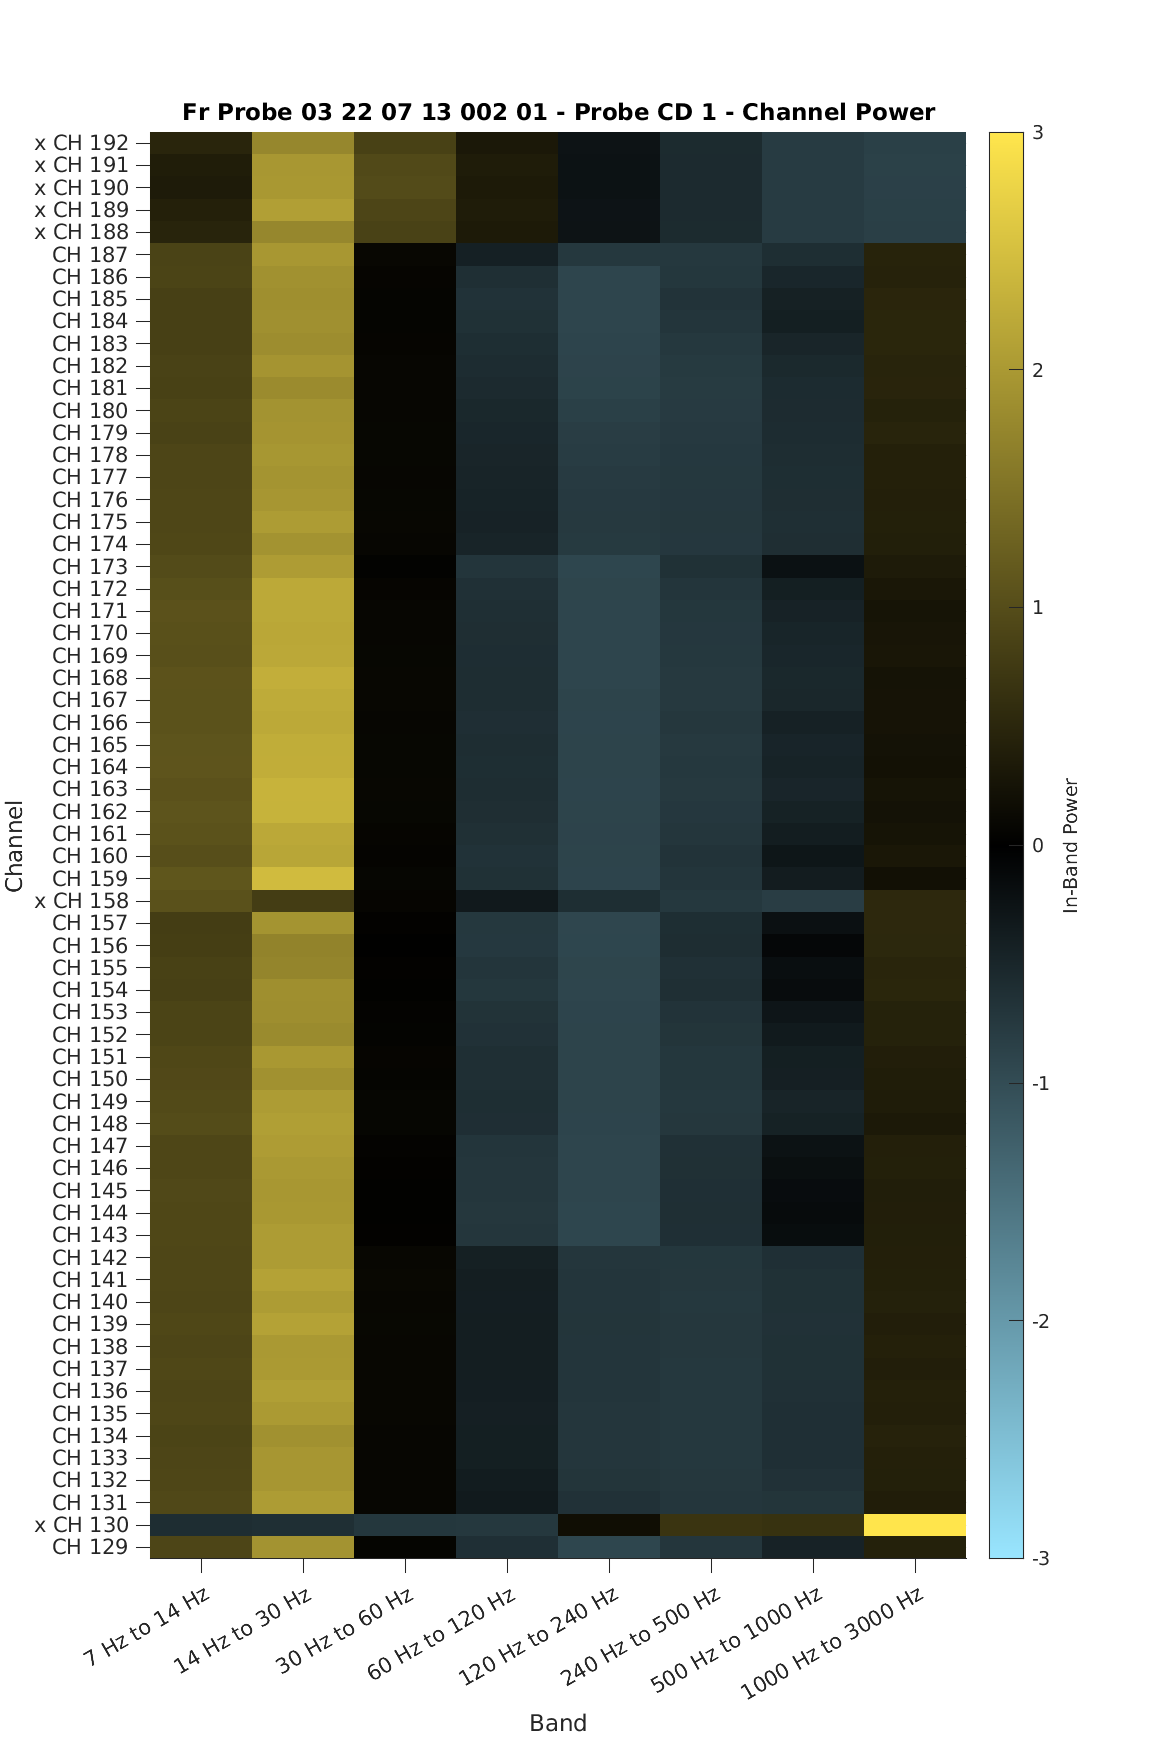
\includegraphics[width=3in]{plots/0713-prCD1-inband-normband} \\
\end{tabular}
%
\end{center}
%
\vfill
{\tiny \input{../LICENSE.md}}
%
\clearpage
%
%
% Front matter.
%
% NOTE - Putting the overview before the TOC!
%
\pagestyle{plain}
\pagenumbering{roman}
\setcounter{page}{1}
%
% Preprocessing pipeline libraries - Library reference - Overview
% Written by Christopher Thomas.

% Dummy out chapter; this is now front-matter.
\iffalse
%
\chapter{Overview}
%
\else
%
\vspace*{0.75in}
{\Huge \bfseries Overview}
\vspace*{\baselineskip}
\label{sect-over}
%
\fi

This is a set of libraries written to support preprocessing of ephys data
collected by Thilo's lab.

The library routines are intended to cover the following tasks:
\begin{itemize}
\item Reading experiment metadata.
\item Reading raw ephys data, game data, and gaze data.
\item Segmenting experiment data into per-trial records.
\item Performing artifact rejection on ephys data.
\item Assisting bad channel detection for ephys data.
\item Producing per-trial records with derived ephys signals (MUA, LFP, etc).
\end{itemize}

% FIXME - Update this later!
Not presently implemented but within the scope of this project:
\begin{itemize}
\item Performing filtering and cleanup of gaze data.
\item Saving per-trial gaze data in Field Trip format.
\end{itemize}

The idea is to make it easy and fast to write pre-processing code so that
effort may be focused on analysis of ephys and behavior data after
pre-processing.

Libraries are provided in the ``\texttt{libraries}'' directory. With that
directory on path, call the \linebreak ``\texttt{addPathsExpPreproc}''
function to add sub-folders.


The following sets of library functions are provided:
\begin{itemize}
%
\item \textbf{``\texttt{epIter}''} functions (Chapter \ref{sect-iter})
are functions intended to perform various preprocessing steps for each
session/probe/trial, and a top-level entry-point function
(\texttt{epIter\_processSessions.m}) that calls these helper functions.
Further documentation is provided in Chapter \ref{sect-iter-notes}.
%
\end{itemize}

The following sample code is provided (in the ``\texttt{code-examples}''
folder):
\begin{itemize}
%
\item \textbf{``\texttt{do\_config.m}''} --
Specifies where to find raw datasets, specifies configuration information
for each of the preprocessing operations.
%
\item \textbf{``\texttt{do\_sessionmeta.m}''} --
Reads eyphs headers and auxiliary (game) files, builds event lists and trial
definitions, and saves all of this metadata in a consolidated format.
%
\item \textbf{``\texttt{do\_preproc.m}''} --
Reads the raw ephys datasets, performs several preprocessing steps, and
saves the results of each step in Field Trip format. Preprocessing steps
are segmentation into trials, artifact removal, bad channel detection,
and filtering, rectification, and downsampling to produce derived signals.
%
\item \textbf{``\texttt{do\_epoch.m}''} --
Reads per-trial Field Trip files, time-aligns them to desired events, and
crops them to a region of interest around these events.
%
\item \textbf{``\texttt{do\_manual\_badchans.m}''} --
Manually specifies bad channels. These can be used instead of automatically
detected bad channels by changing a configuration flag in
\texttt{do\_config.m}.
%
\end{itemize}

To run the sample analysis code:
\begin{itemize}
\item Make sure that the configuration file points to the FLToken dataset.
\item Make sure that all needed libraries are on Matlab's search path, or
are available via the symbolic links in the ``\texttt{libs-ext}'' folder.
\item If using ``\texttt{make}'' from the Linux or MacOS command line:
\begin{verbatim}
make allclean
make session
make preproc
make epoch
\end{verbatim}
\item To run from within the Matlab GUI:
\begin{itemize}
\item Make sure the ``\texttt{data-sessions}'', ``\texttt{data-trials}'',
``\texttt{data-epoched}'', and ``\texttt{plots}'' folders exist.
\item Run the following commands:
\begin{verbatim}
do_sessionmeta
do_preproc
do_epoch
\end{verbatim}
\end{itemize}
\item Plots will be produced by the pre-processing script (bad channel
analysis plots) and by the epoching script (strip-chart plots of timelocked
signals and of selected individual trials). Use ``\texttt{make gallery}''
from the Linux or MacOS command line to build a gallery web page showing
these pictures, if desired.
\end{itemize}

%
% This is the end of the file.

\clearpage
%
\tableofcontents
\clearpage
%
%
% Document parts.
%
\pagestyle{plain}
\setcounter{page}{1}
\pagenumbering{arabic}
%
\part{Examples}
\label{sect-samples}
%
\input{epp-libs-sample-preproc}
%
\part{Library Functions}
\label{sect-libs}
%
\input{epp-libs-iter-notes}
\input{epp-libs-iter}
%
%
\end{document}

%
% This is the end of the file.
